
早期计算机的编程非常困难,因为处理器慢、内存有限、编译器差劲,完成一个程序需要花费大量的时间。开发者必须知道CPU的架构,内存的布局,对于当时的编译器,关键的代码必须用汇编来写。

后来情况有所好转了。处理器的速度越来越快,编译器开发者使用了一些使程序更快的技巧,所以曾经需要巨大硬盘容量的处理器,现在的所需的容量也就一个普通PC机主存的大小,开发者可以花更多的时间来解决实际问题。这反映在编程语言和设计风格上:在高级语言和不断发展的设计和编程实践之间,开发者的重点从他们想在代码中\textbf{说什么},转变为到他们想\textbf{怎么说}。

以前的常识,如CPU到底有多少寄存器,寄存器的名字都是什么,现在却变成了一个深奥且还有些难懂的话题。曾经的“大型代码库”是指需要用双手才能托起,而现在已经完全在版本控制系统的掌握之下了。几乎不需要为特定的处理器或内存系统编写特定的代码,可移植的代码越来越流行。

对于手动汇编编程,实际上很难超越编译器生成的代码。当代码量增加,大多数开发者无法自行完成手动汇编。对于应用程序和编写者来说,有“足够的性能”即可,开发者需要对其他方面的事情更加关注(需要明确的是,开发者可以专注于代码的可读性,而不必担心添加一个名称有意义的函数是否会使程序慢)。

然后,也算是老生常谈,“性能的自增长”的时代结束了。看似不断增长的计算能力的提升只是在程序性能方面……停止了。


\hspace*{\fill} \\ %插入空行
\begin{center}
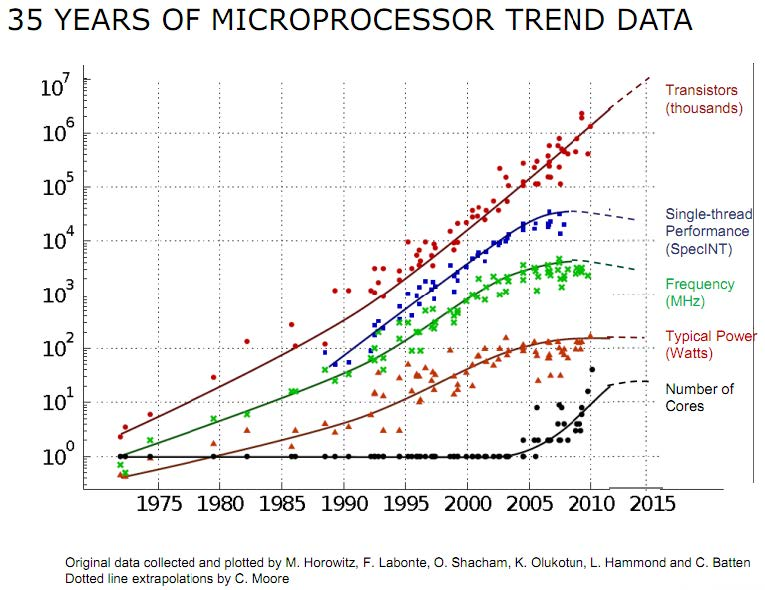
\includegraphics[width=0.9\textwidth]{content/1/chapter1/images/1.jpg}\\
图1.1 -微处理器35年的发展历程 \\
(引用于 \url{https://github.com/karlrupp/microprocessor-trend-data and https://github.com/karlrupp/microprocessor-trend-data/blob/master/LICENSE.txt})
\end{center}

在2005年左右,单个CPU的计算能力达到饱和。在很大程度上,这与CPU频率直接相关,CPU频率也停止增长。反过来,CPU的频率又受到几个因素的限制,其中之一是功耗(如果频率趋势保持不变,如今的CPU每平方毫米的功率将超过将火箭送入太空的大型喷气式发动机)。

从前面的图表中可以明显看出,并不是所有的进步指标都在2005年停滞不前:集成在单个芯片中的晶体管数量一直在增长。那么,如果不是让芯片更快,他们在做什么呢?答案是双重的,下面的曲线揭示了其中的部分原因:设计师没有将单个处理器做得更大,而是将多个处理器核心放在一起。当然,所有这些处理器的计算能力会随着核的数量而增加。“晶体管之谜”的第二部分(晶体管都到哪里去了?)中,硬件设计师对处理器功能进行了各种增强,这些增强可以用来提高性能,但也需要开发者知道如何使用它们。

我们刚才了解到的处理器的变化是并发编程进入主流的原因,但这种变化的意义远不止于此。本书中为了获得最佳性能,开发者需要理解处理器和内存体系结构,及其间的交互,所以出色的表现不再是“偶然发生”。与此同时,我们在编写代码时所取得的进步,也清楚地表达了需要做什么,而不是如何做。我们仍然希望编写可读和可维护的代码,并且(不是但是)这些代码是高效的。

可以肯定的是,对于许多应用程序来说,现代CPU的性能已经足够,但程序的性能比过去有了更多的关注,这在很大程度上是因为CPU的变化。因为我们想要在不一定能获得最佳计算资源的应用程序中做更多的计算(例如,今天的便携式医疗设备可能有一整个神经网络程序在其中工作)。

幸运的是,我们不必在黑暗的储藏室里翻找一堆堆腐烂的穿孔卡片来重新学习那些古老的艺术形式。任何时候,都有困难的问题,对于许多软件开发者来说,计算能力永远不够用这句话完全正确。随着计算能力呈指数级增长,对它的需求也在相应的增长(古老的艺术只会在少数需要它的领域中得以延续)。











